\chapter{Analysis}
\section{Abstract}
As I am an A Level Maths (with mechanics) and Physics student, I have studied the topics of projectile motion and radioactive decay. I myself found these topics to be difficult as did many of my peers. The current method of practising mathematics and physics questions is to attempt problems from a course textbook. As there are many questions for the student to try, they can seem repetitive or boring causing the student to be more likely to stop. This can be solved by providing a range of questions to provide variety. The majority of problems are provided with no diagram, so the student has to interpret the text and potentially draw their own diagram. While this type of question is likely to come up in the exam, when the student is first learning the topic, it is important that they understand the topic fully before attempting harder, exam style questions. This can be solved by providing diagrams for the student. This allows the question text to be represented visually which make the problem easier to understand, and it will allow the student to relate the question to the underlying concepts that they are learning.

This software will be an easy to use platform. It will generate questions from the projectile motion and radioactive decay topics, and will draw graphs to go with these. The main aim of the software is to be a learning tool, to help students understand the basics of these topics.
\section{Features of the proposed solution that can be solved using computational methods}
\subsection{Random nature of questions}
The questions will be randomly generated. The base question will be stored so that there are elements within it that can be changed. This allows a loop to be created, which will produce \textit{n} amount of questions, with the elements being changed to a random number from a specified range. The generated elements can then be used to create the diagram or graph, by putting these elements into the diagram generation function.
\subsection{Answer Verification}
The number of significant figures in the student's answer will not matter. If the student's answer is the same as the calculated answer to any number of significant figures it will be marked as correct. Computationally, this can be implemented by using built in \textbf{round} functions, meaning that the mathematics behind this does not have to be coded from scratch. This will be faster than if this was implemented non-computationally.
\subsection{Generation of diagrams}
For both projectile motion and radioactive decay, graphs can be generated using an iterative method. This works by supplying an equation with a variable that can be incremented. This is usually time \textit{t}. The equation then outputs a value that plotted as the y coordinate on a graph, with the x coordinate being the time value inputted into the equation. This solution will enable graphs of projectile motion and radioactive decay to be quickly generated for display.
\section{Stakeholders}
Students studying A Level physics are the main target users of this program. It will offer an unlimited supply of questions to practice outside of the textbook. The questions will be provided with a graph or diagram which could make the question seem easier to some. This is intended, as the program is meant to aid understanding of the fundamentals of these topics. 
A Level physics teachers are another target group. They will be able to use this tool in initial lessons to demonstrate how to answer these type of questions. The generated graph will enable easy explanation of the question, and will save time for the teacher. Once the basics have been covered, teachers could task students to complete questions on the application.
\clearpage
\section{Existing Solutions}
\begin{figure}[h]
	\centering
	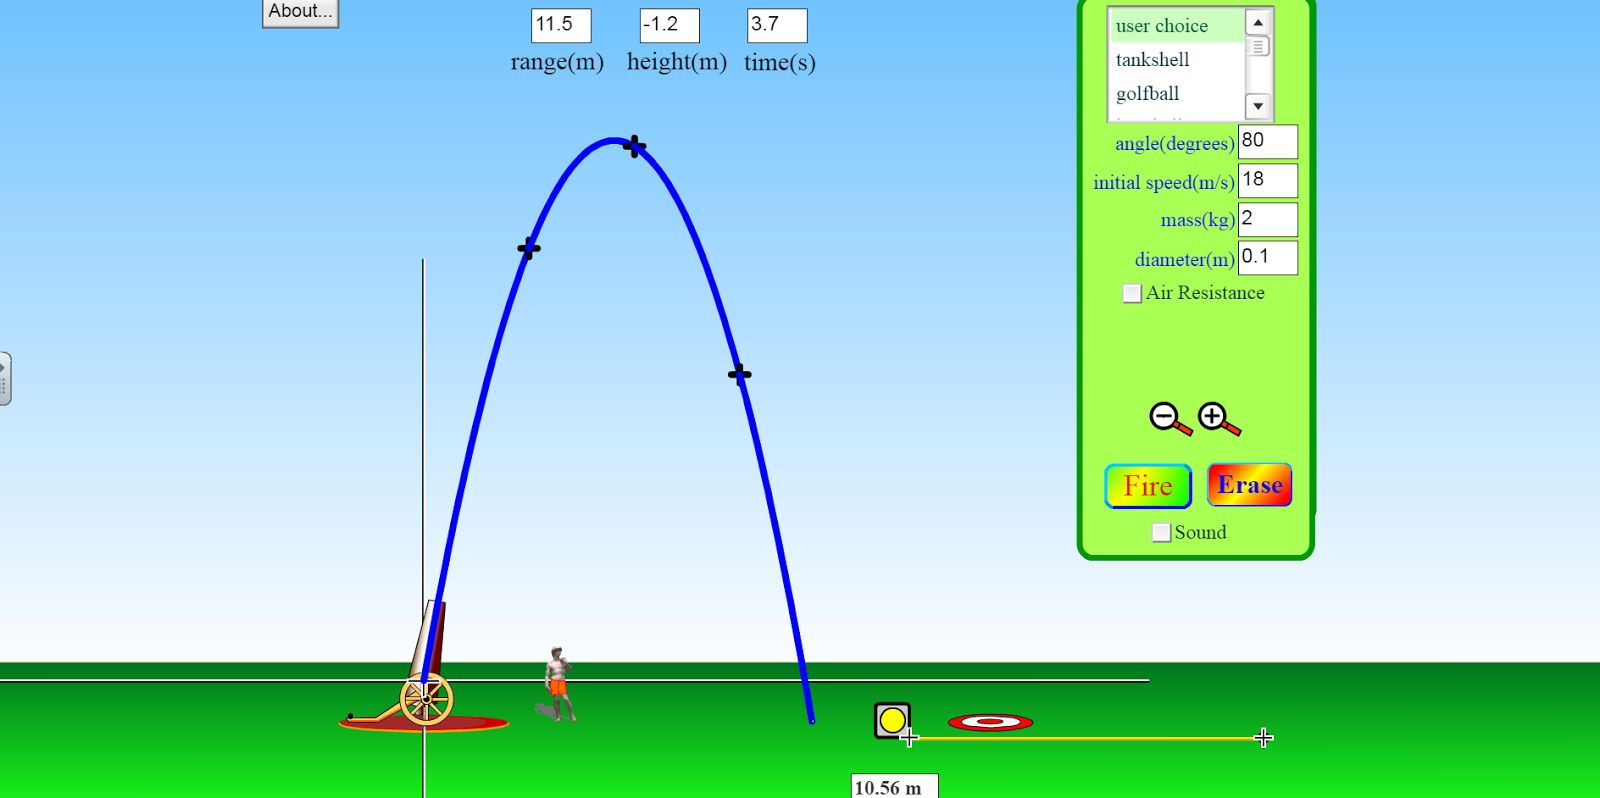
\includegraphics[width=\textwidth,height=\textheight,keepaspectratio]{Analysis-000}
	\caption[PHET Interactive projectile motion simulator.]{PHET Interactive projectile motion simulator. \autocite{phet}}
	\label{phet}
\end{figure}
This piece of software display the path of an object fired out of a cannon. You can modify the mass and diameter of the object being fired. This will only change the motion of the object if air resistance is being simulated. This simulation does have an option to enable air resistance, which will provide a more realistic simulation. However air resistance is not taken into account in the A Level Physics exam, so this feature will be left out. The launch speed and angle can also be changed. The graph generation should have changeable parameters, so that the values in the question can be used to produce a graph of itself. The user won't be allowed to directly change these values, as this is a question generation program, not a sandbox.
\clearpage
\begin{figure}[h]
	\centering
	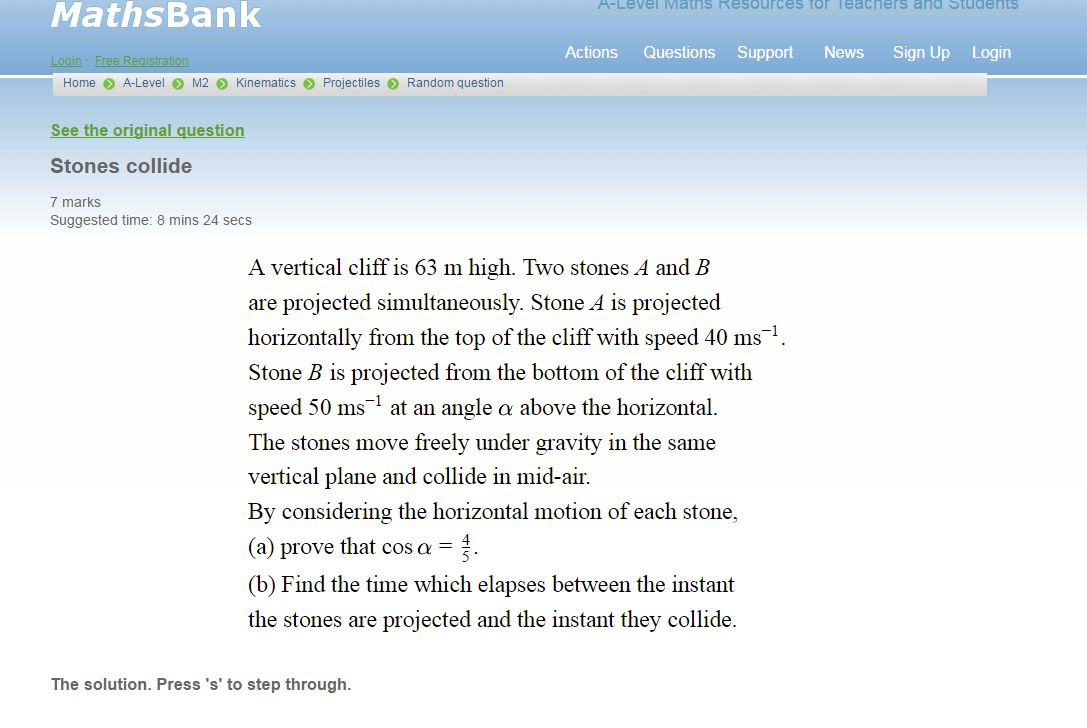
\includegraphics[width=\textwidth,height=\textheight,keepaspectratio]{Analysis-001}
	\caption[MathsBank M2 Projectile motion question bank.]{MathsBank M2 Projectile motion question bank.
	 \autocite{mb}}
 	\label{fig:mb}
\end{figure}
This is an example of an exam style question. The question provides good context, making it easy to understand. A diagram is not provided, as it is expected that the student draws one for themselves. This type of question is not aimed at people just starting the topic, so the style of the question would have to be changed so that all of the information required is displayed obviously, rather than it being hidden in the text.
\clearpage
\begin{figure}[h]
	\centering
	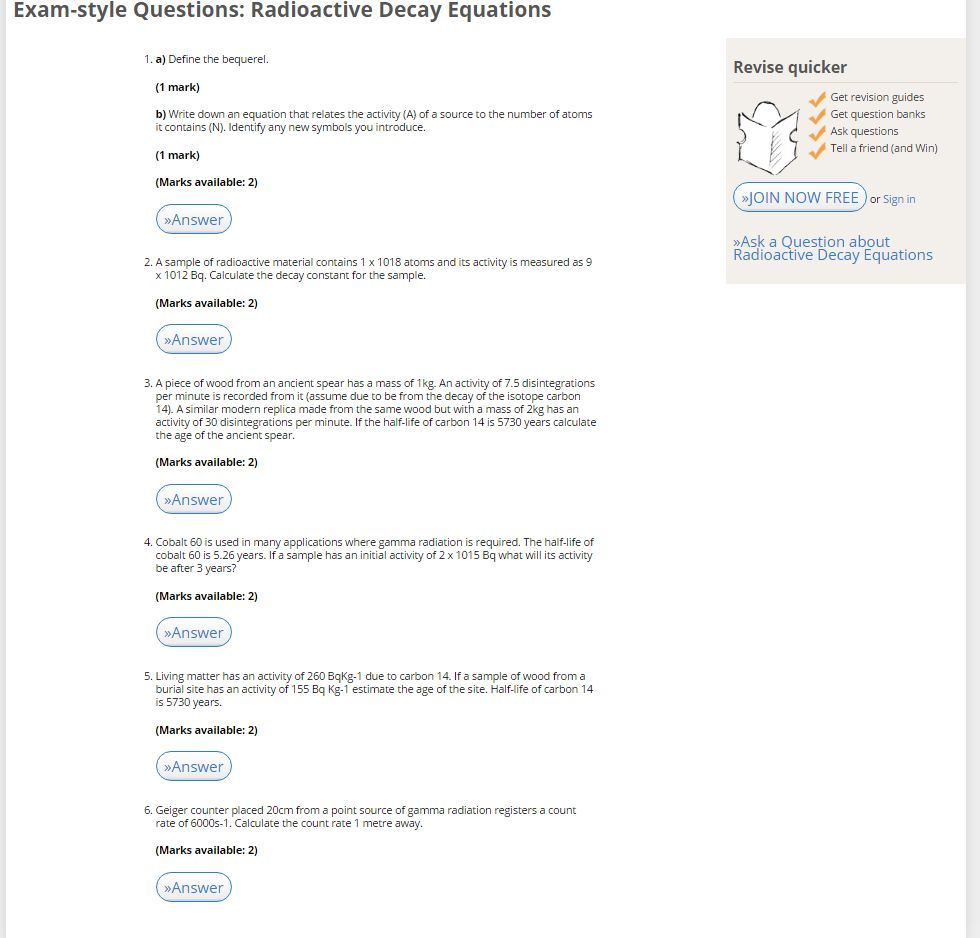
\includegraphics[width=\textwidth,height=\textheight,keepaspectratio]{Analysis-002}
	\caption[Exam-style Questions: Radioactive Decay Equations.]{Exam-style Questions: Radioactive Decay Equations. \autocite{scool}}
\end{figure}
These questions are extensive, and with a realistic context, making it more approachable to the student. Some of the questions are not suitable for random variation like Question 1, which are purely fact recall questions. The style of the other questions are ideal, as they are not too complex, and allow a graph or diagram to be drawn based on the information in the question.
\section{Solution}
\subsection{Question generation}
\subsubsection{Projectile motion}
The structure of the questions generated will be based on the MathsBank questions seen in Figure \ref{fig:mb}. The length of the question will be much shorter, only containing one part. This will avoid boredom from similar questions, and will avoid problems with the student having to remember answers to previous parts in order to correctly solve the next part. 
\begin{figure}[h]
	\centering
	A ball is projected with speed \(x \text{ ms}^{-1}
	\). At the starting point the ball is \(S\) m off the ground. The highest point of the ball is \(y\)  m.
	\caption{Example projectile motion question.}
	\label{expm}
\end{figure}
Figure \ref{expm} shows an example question, which is the style that will be generated for the user. The parameters which will be changed \(x, S \text{ and } y\) are obvious to the user, and no extra calculations are required. All of the information required to answer the question is easily shown in the question.
\subsubsection{Radioactive Decay}
The questions used in the program will be very similar to the questions found on S-cool\autocite{scool}. The only changes will be that the fact recall questions will be removed, due to that fact that these can't be truly randomised.
\begin{figure}[h]
	\centering
	A sample of radioactive material contains \(n\) atoms and its activity is measured as \(x\) Bq. Calculate the decay constant for the sample.
	\caption{Example radioactive decay question.}
	\label{exrd}
\end{figure}

Again, this shows how easy it is to randomise the question, with only the letter variables in Figure \ref{exrd} having to be changed.

\subsection{GUI}
The GUI\footnote{Graphical User Interface.} for the two different topics will be very similar, as they both have three distinct elements:	
\begin{itemize}
	\item{Question box}
	\item{Graph or diagram}
	\item{Answer box} 
\end{itemize}
The graph or diagram generated will be based on \ref{phet}, but it will be a much simpler version of this. Only two colours will be used, which will reduce confusion, and avoid distraction. There will also be no representation of the object being fired for clarity.
\section{Justification}
Random question generation was chosen after looking at the questions from MathsBank \autocite{mb} and SCool \autocite{scool} it is obvious that there is only a limited amount of questions available, and that after about an hours use there would be no questions left, meaning that it is useless. The choice to randomise the questions therefore seems very logical, as it will extend the time that the program is useful for.

Generating a graph to go along with the question was chosen to make the question seem less intimidating. From looking at Figure \ref{fig:mb} the question looks very intimidating. This is because diagrams must be drawn by the student, and extra calculations must be made to get information required to answer the question, or it must be inferred from the question. This is shown clearly in Figure \ref{fig:mb}, where the information is not shown directly, for example instead of giving $\theta$ they give cos $\theta$ which is confusing.
\section{Essential Features}
\begin{itemize}
	\item{Functional GUI Menu.}
	\item{Clear distinction between topics to avoid confusion.}
	\item{Questions with random variables.}
	\item{Simple random variables that are realistic for the question type.}
	\item{Verification of student's answer. Answer is accepted to any amount of significant figures.}
	\item{Graph or diagram to supplement question.}
\end{itemize}
\subsubsection{Functional GUI Menu}
This is to make the software easy to use. The user should be able to use the program with no instruction, so it must be intuitive. By designing like this, the user is more focussed on answering the questions, than trying to use the program.
\subsubsection{Clear distinction between topics to avoid confusion}
This follows on from the functional GUI.  A clear distinction will simplify the experience for the user, and will allow the student to target their question practice to a specific topic.
\subsubsection{Simple random variables that are realistic for the question type}
By making the variables simple, i.e a number with no decimals places, it makes the question easier to read and more like it would be in an exam. If they are realistic, it gives the question more context so is more interesting to the student.
\subsubsection{Verification of student's answer}
It is important that the student knows whether they got the question right, as it worthless otherwise. The decision to make the student's answer be accepted to any amount of significant figures, is so that they don't get confused if there answer is marked wrong because of an incorrect amount of significant figures.
\subsubsection{Graph or Diagram}
The graph or diagram is important as it makes the question easier to understand. This is important, as the idea of the program is to provide a platform to practice and understand the basics of the topics.

\section{Limits of proposed solution}
The main issue with this solution is that the questions won't be truly random. This is because only parts of the question are randomised. For example looking at Figure \ref{expm} and \ref{exrd} only the letter variables are randomised. There will be a small number of base questions, which determine the style of question and this cannot be randomised as it is out of the scope of this project. For the target user of this program, this won't be a problem. They won't be using the program for too long, as they will learn the basics and then move on to harder questions. In the time that it takes to do that, they won't have time to just learn how to answer the specific type of question, instead of learning the theory behind the question.

\section{Project Requirements}
\subsection{Programming language}
Python 3.5 will be the main project requirement as it is the programming language that the software will be written in. This language is being used because of the great number of libraries available to make the development process easier, and because it is portable, so can run on any modern computer.
\subsection{GUI}
To create the GUI, PyQt will be used, which is a python wrapper for QT. Qt is a cross-platform application framework that is used for developing application software that can be run on various software and hardware platforms with little or no change in the underlying codebase\autocite{qt}.This library will allow portability, and the code won't have to be rewritten due to it being a Python wrapper. Qt comes with a WYSIWYG\footnote{What you see is what you get.} editor called QtCreator, which is similar to the Visual Basic form designer. A GUI can be easily created using this, as it can be made visually, instead of having to make it in code, which is time consuming and can be hard to get right. Once the GUI is made in QtCreator, PyUIC5 can be run to convert the Qt code into Python code which can be used to display the GUI.
\subsection{Graph generation}
Matplotlib\footnote{Python Library used for plotting graphs.} will be used to generate the graph and diagram for display on the GUI. It is easy to use, and executes quickly, which is important to reduce waiting time for the user. The matplotlib window will not be shown directly to the user, matplotlib will be called to generate an image of the graph which will then be displayed. This is to make sure that there is no issues with graph size.
\subsection{Hardware requirements}
The only requirement is a relatively modern PC, that is running a contemporary operating system. Greater than 2 gigabytes of RAM, and a CPU clock speed greater than 2Ghz is recommended so the questions are displayed promptly.
\subsection{Final Build}
The final build of the software will have a .exe file that will be run by the user. The Python libraries still need to be available to the program, so they need to be installed on the computer. This can be done in two ways, either by installing the Anaconda Python distribution, or providing a virtualenv\footnote{An isolated Python environment} with the libraries installed. A virtualenv would be easier for the user, as they don't have to install any additional software.
\section{Success Criteria}
\begin{itemize}
	\item It should have a functional, easy to use GUI.
	\item It will have randomly generated questions
	\item It should have realistic values in the question
	\item Random question should be shown to the user within a second of page display
	\item Graph or diagram will be generated in relation to question
	\item Graph should be displayed within a second
	\item Student's answers should be verified no matter the amount of significant figures.
\end{itemize}